\addsec{Anhang} %addsec erhält keine nummerrierung
\label{sec:anhang} %label erstellen für quervereise

\begin{figure}[h!]
	\centering
	\subfigure[Register A]{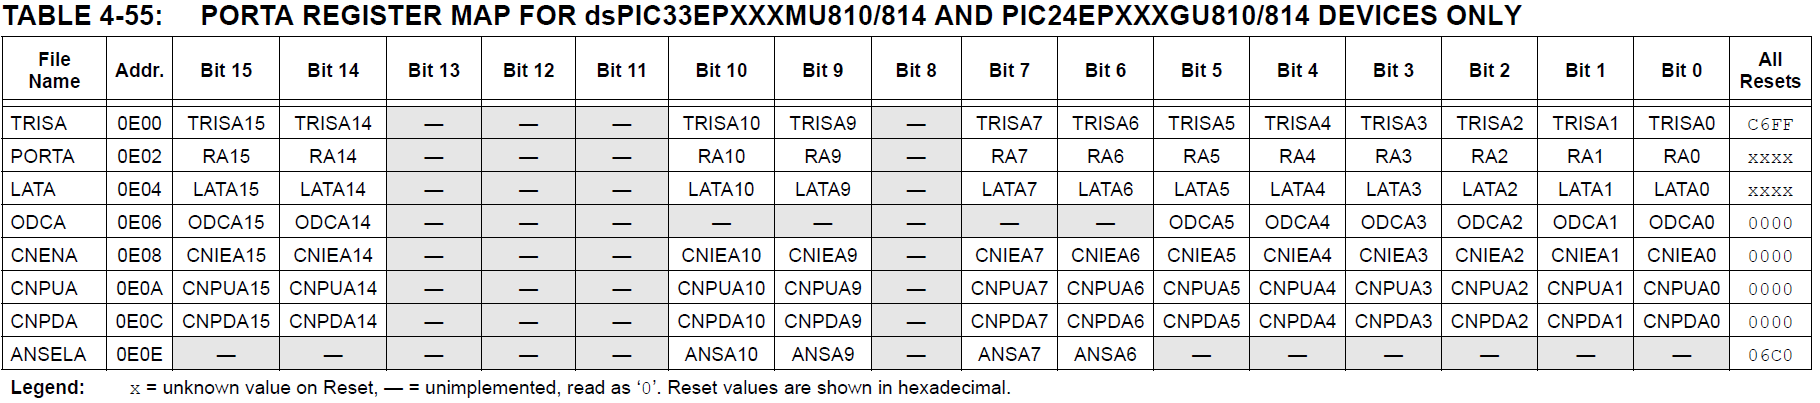
\includegraphics[width=0.8\textwidth]{Images/PORTA}} 
	\subfigure[Register B]{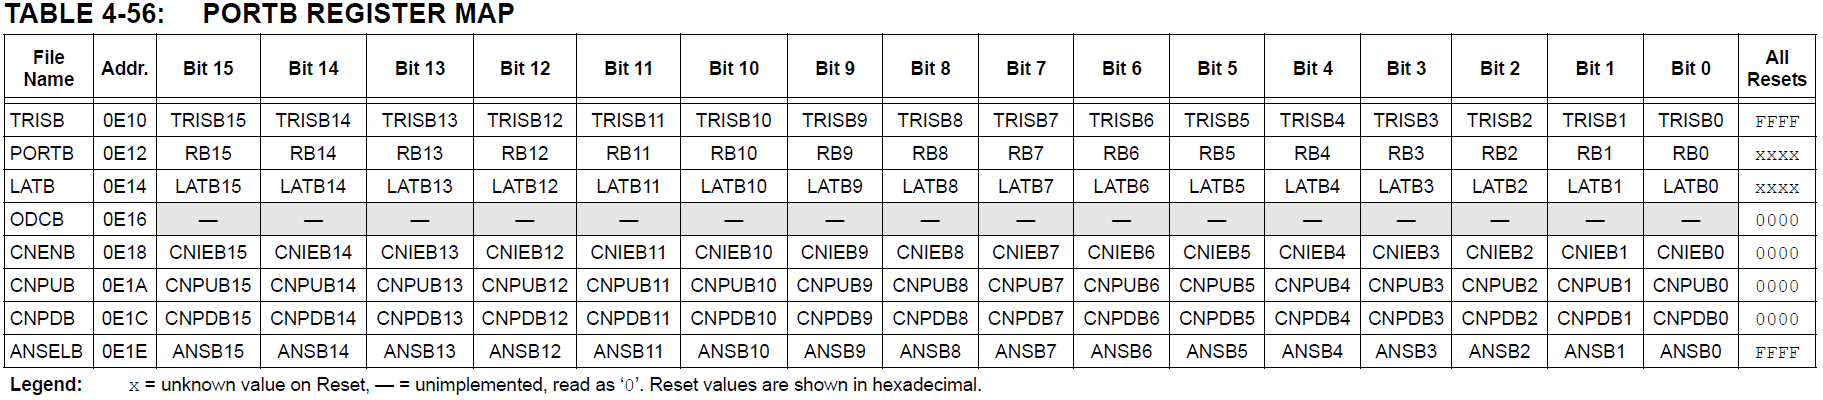
\includegraphics[width=0.8\textwidth]{Images/PORTB}} 
	\subfigure[Register C]{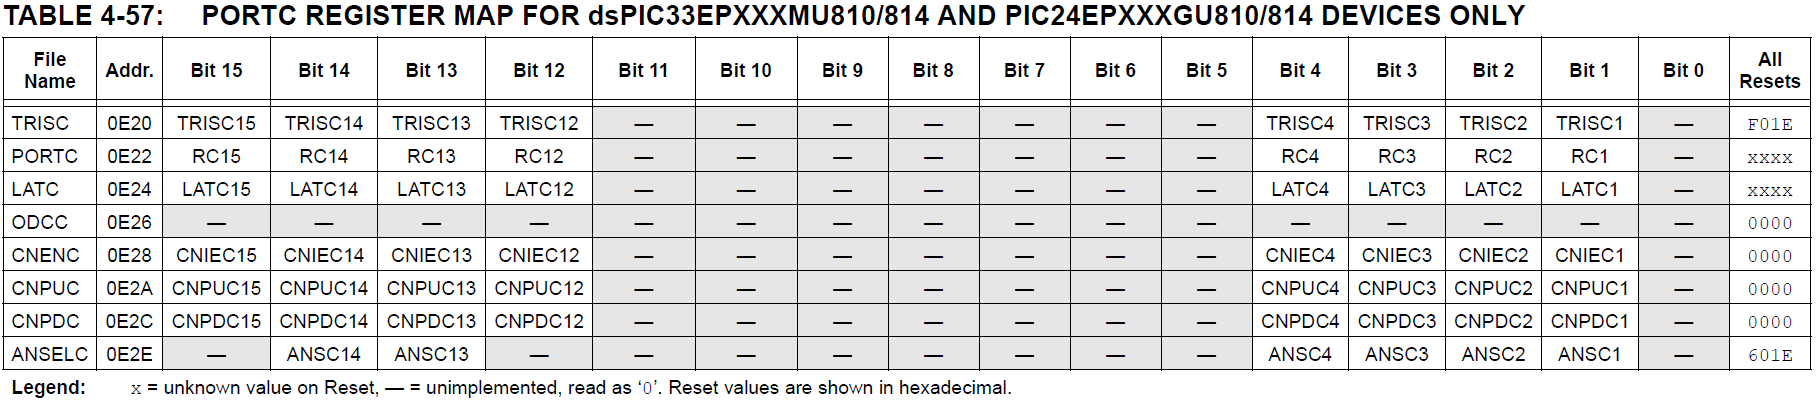
\includegraphics[width=0.8\textwidth]{Images/PORTC}} 
	\subfigure[Register D]{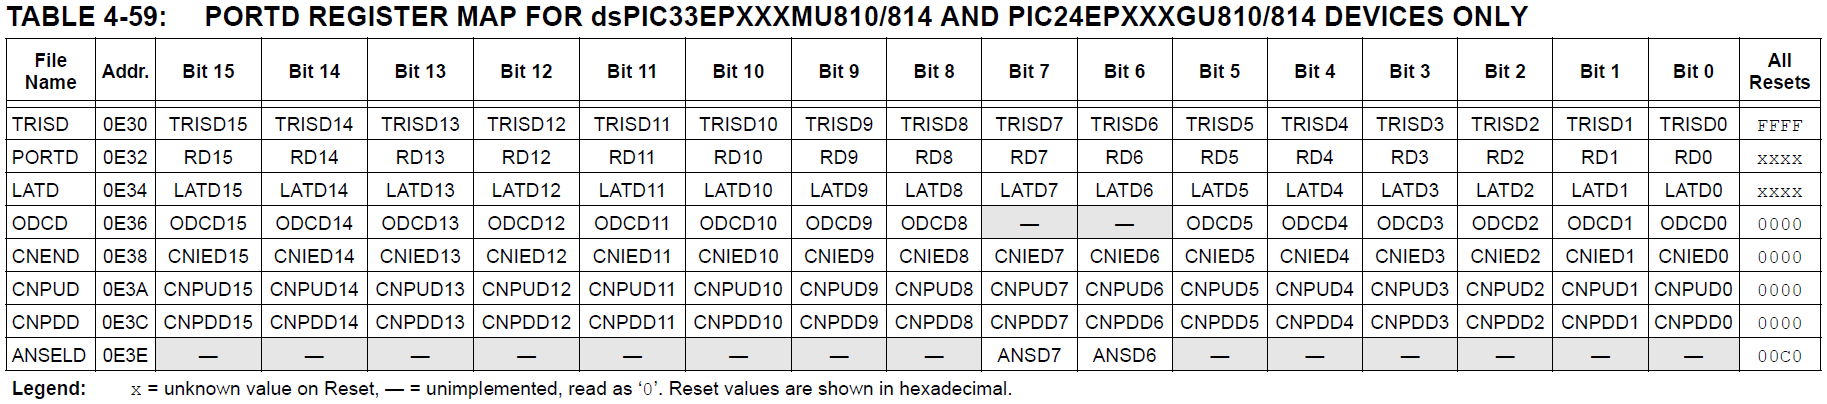
\includegraphics[width=0.8\textwidth]{Images/PORTD}} 
	\subfigure[Register E]{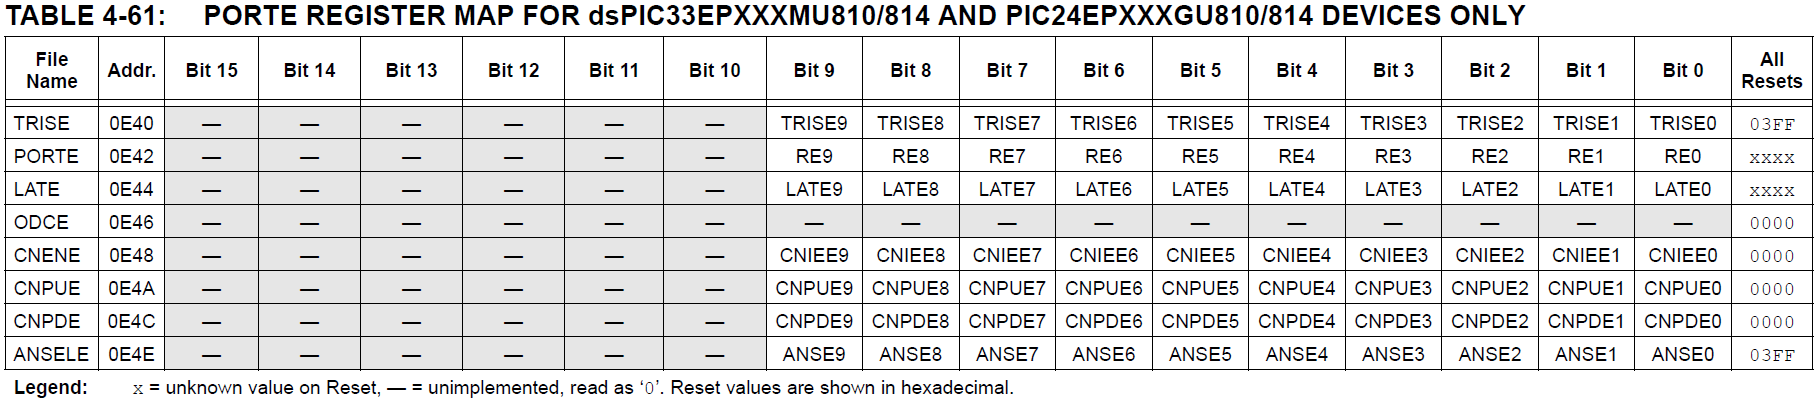
\includegraphics[width=0.8\textwidth]{Images/PORTE}} 
	\subfigure[Register F]{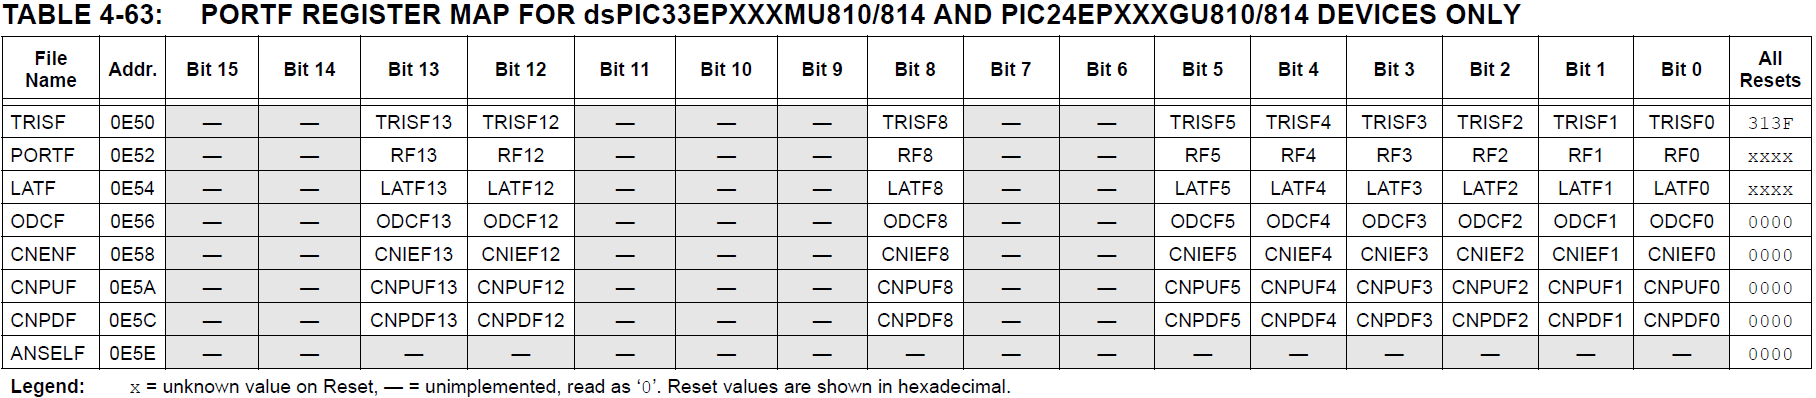
\includegraphics[width=0.8\textwidth]{Images/PORTF}}
	\subfigure[Register G]{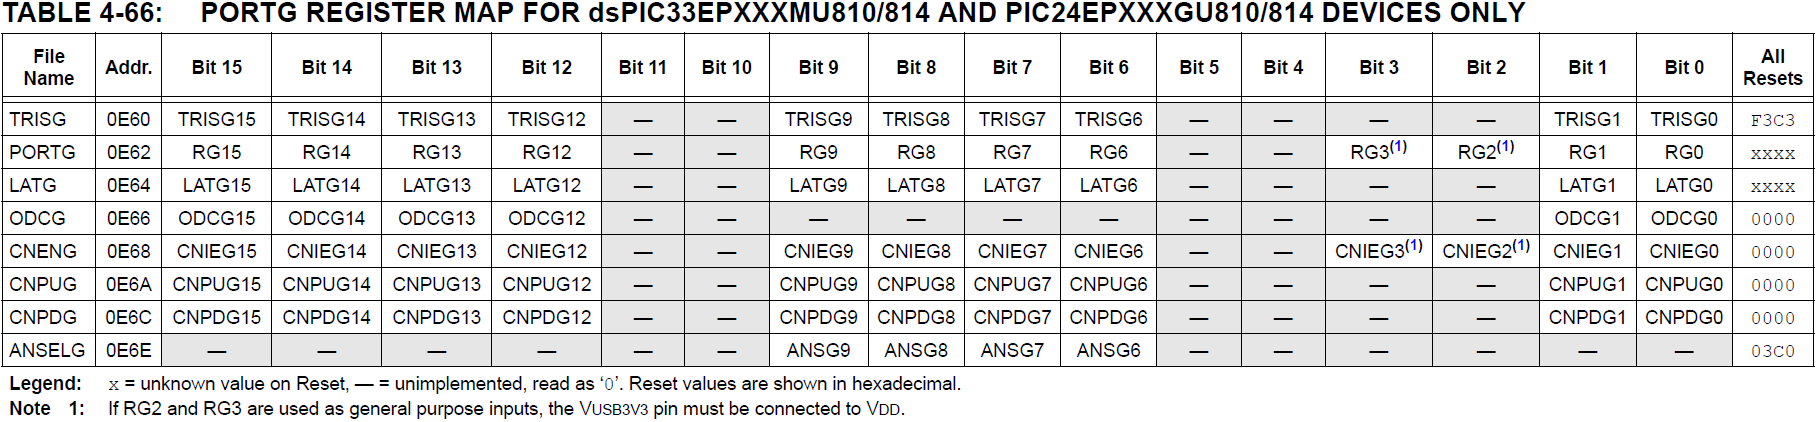
\includegraphics[width=0.8\textwidth]{Images/PORTG}}   
	\caption{PORTA-G Register Map}
	\label{image:PortMap}
\end{figure}

%
%\begin{figure}[h]
%	\centering
%	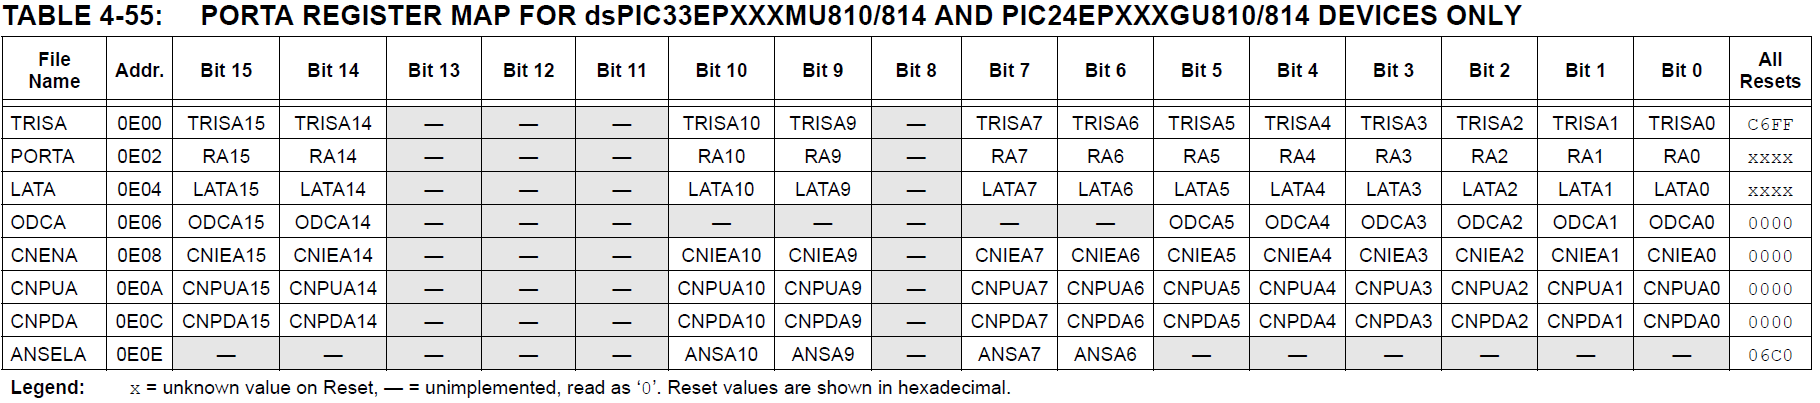
\includegraphics[width=\textwidth]{Images/PORTA}
%	\caption[PORTA Register Map]{PORTA Register Map}
%	\label{image:PORTA}
%\end{figure}
%
%\begin{figure}[h]
%	\centering
%	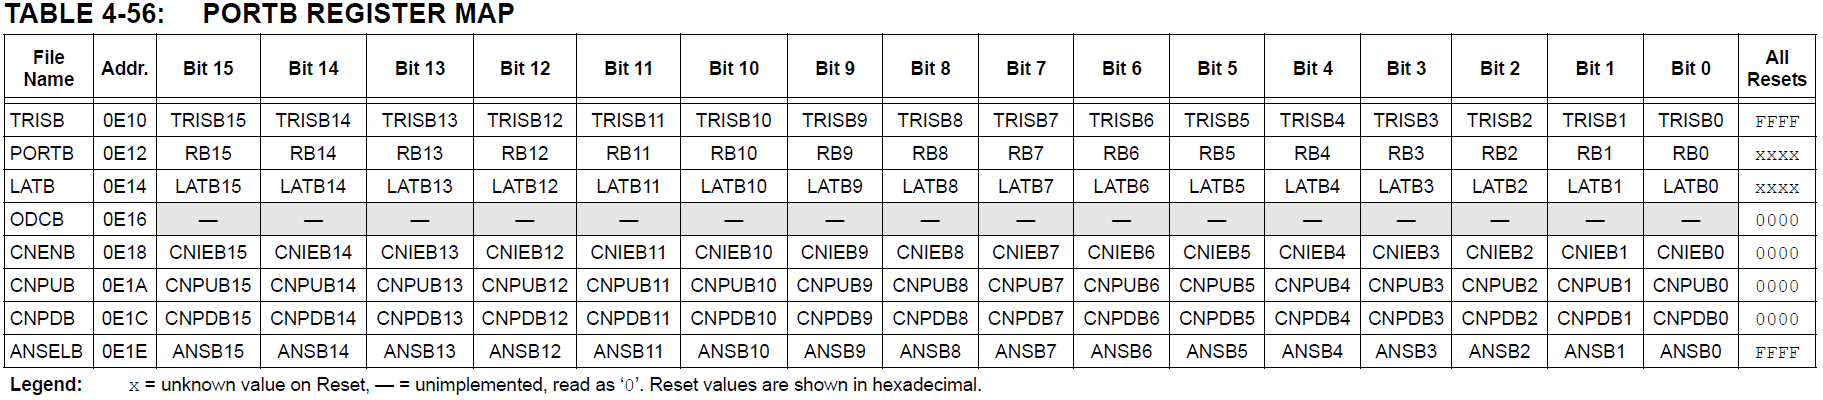
\includegraphics[width=\textwidth]{Images/PORTB}
%	\caption[PORTB Register Map]{PORTB Register Map}
%	\label{image:PORTB}
%\end{figure}
%
%\begin{figure}[h]
%	\centering
%	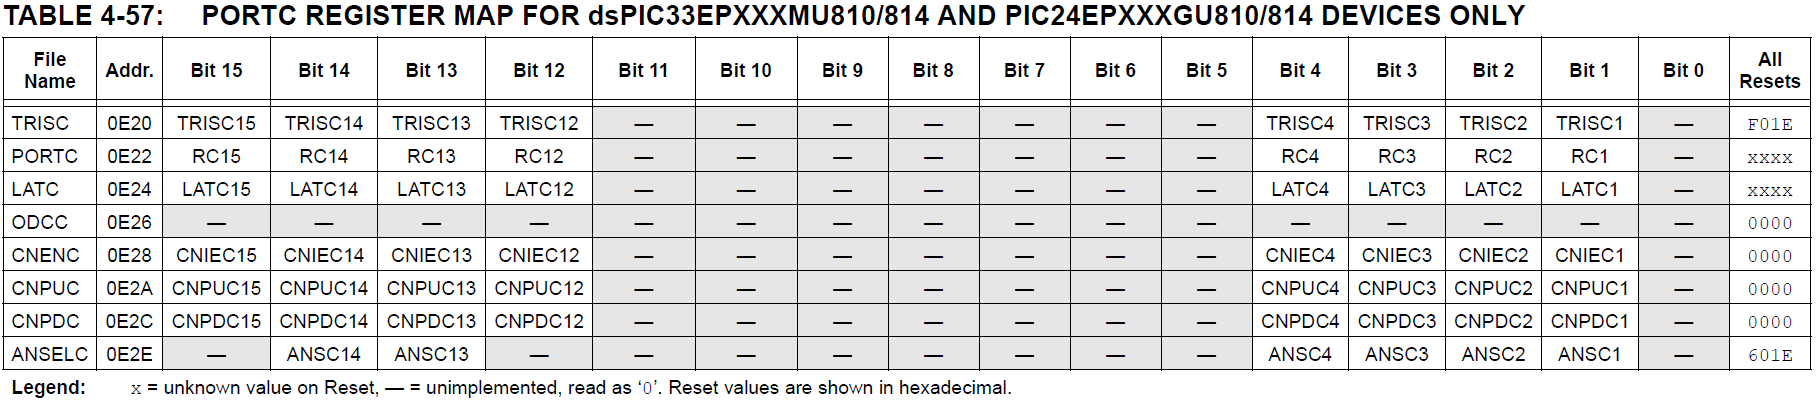
\includegraphics[width=\textwidth]{Images/PORTC}
%	\caption[PORTC Register Map]{PORTC Register Map}
%	\label{image:PORTC}
%\end{figure}
%
%\begin{figure}[h]
%	\centering
%	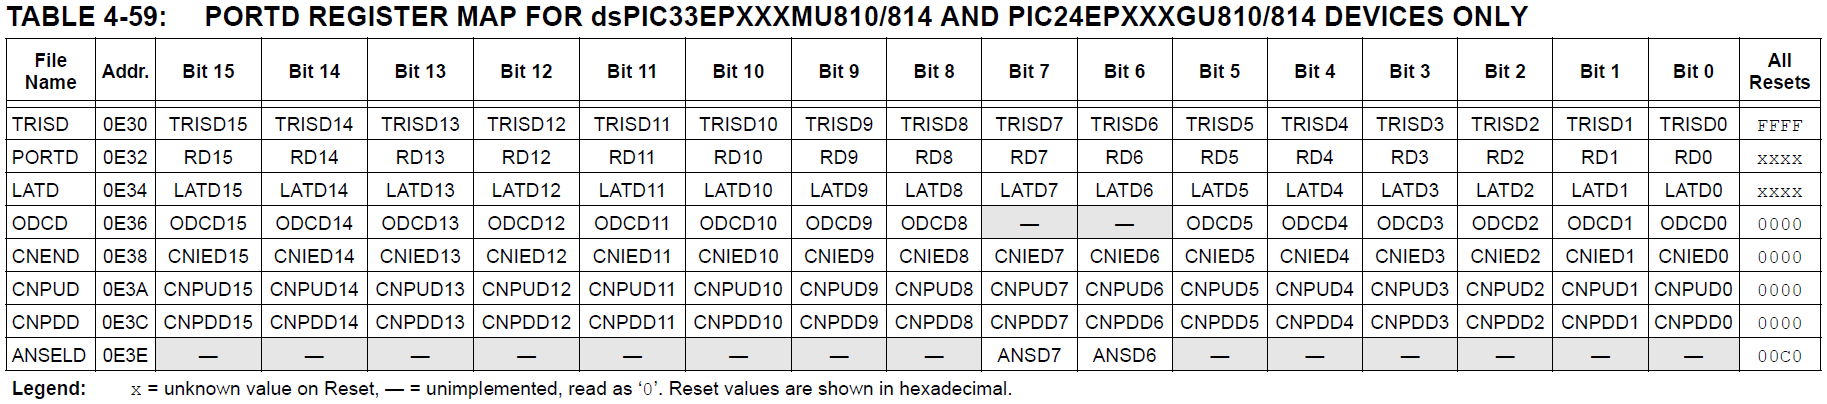
\includegraphics[width=\textwidth]{Images/PORTD}
%	\caption[PORTD Register Map]{PORTD Register Map}
%	\label{image:PORTD}
%\end{figure}
%
%\begin{figure}[!h]
%	\centering
%	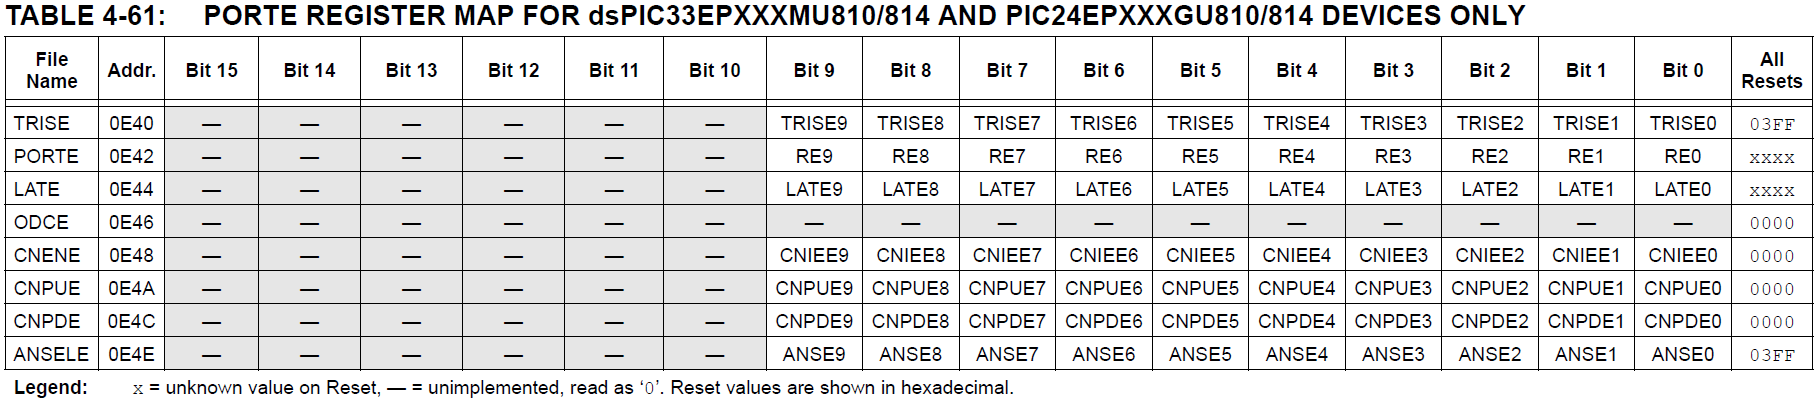
\includegraphics[width=\textwidth]{Images/PORTE}
%	\caption[PORTE Register Map]{PORTE Register Map}
%	\label{image:PORTE}
%\end{figure}
%
%\begin{figure}[!h]
%	\centering
%	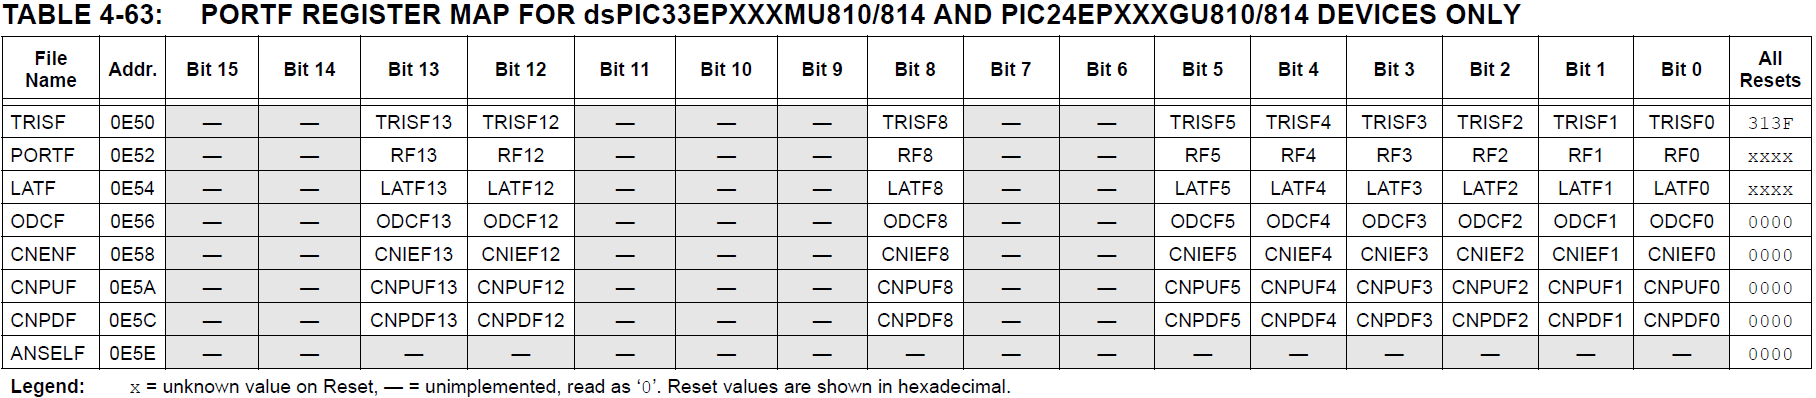
\includegraphics[width=\textwidth]{Images/PORTF}
%	\caption[PORTF Register Map]{PORTF Register Map}
%	\label{image:PORTF}
%\end{figure}
%
%\begin{figure}[!h]
%	\centering
%	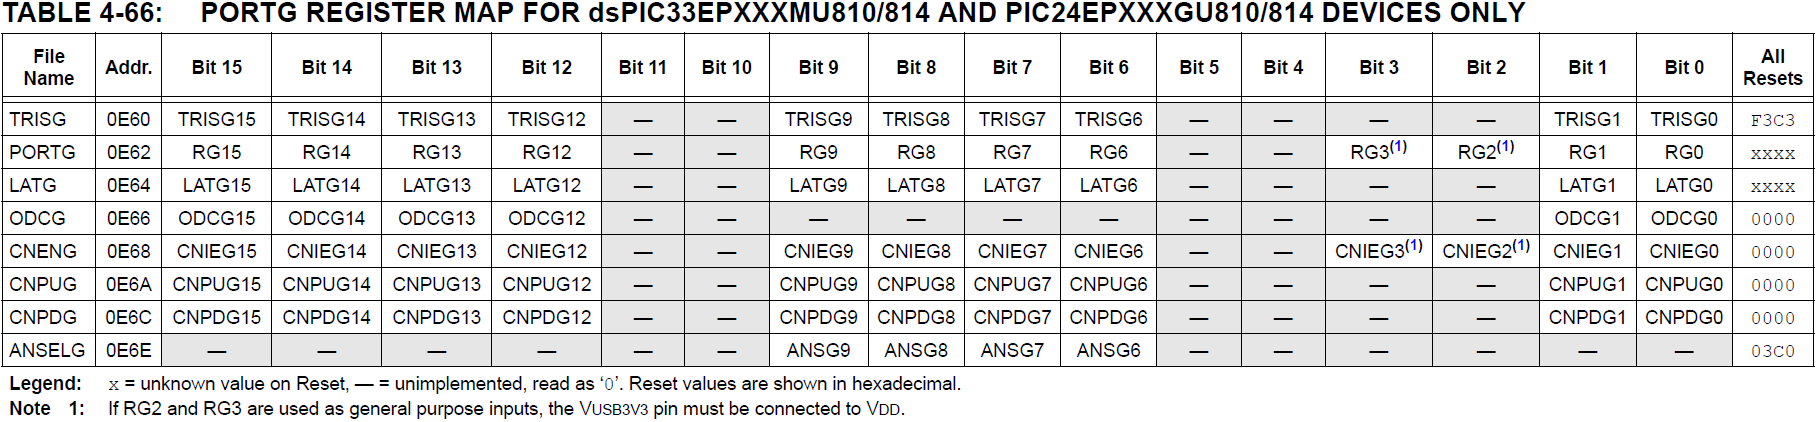
\includegraphics[width=\textwidth]{Images/PORTG}
%	\caption[PORTG Register Map]{PORTG Register Map}
%	\label{image:PORTG}
%\end{figure}

\begin{figure}[!h]
	\centering
	\includegraphics[width=\textwidth]{Images/page207}
	\caption[I/O Ports]{I/O Ports -Datenblatt S.207}
	\label{image:page207}
\end{figure}

\begin{figure}[!h]
	\centering
	\includegraphics[width=\textwidth]{Images/page208}
	\caption[Block Diagramm I/O Ports]{Block Diagramm I/O Ports -Datenblatt S.208}
	\label{image:page208}
\end{figure}	

\begin{figure}[!h]
	\centering
	\includegraphics[width=\textwidth]{Images/page209}
	\caption[I/O Ports]{I/O Ports -Datenblatt S.209}
	\label{image:page209}
\end{figure}

\begin{figure}[!h]
	\centering
	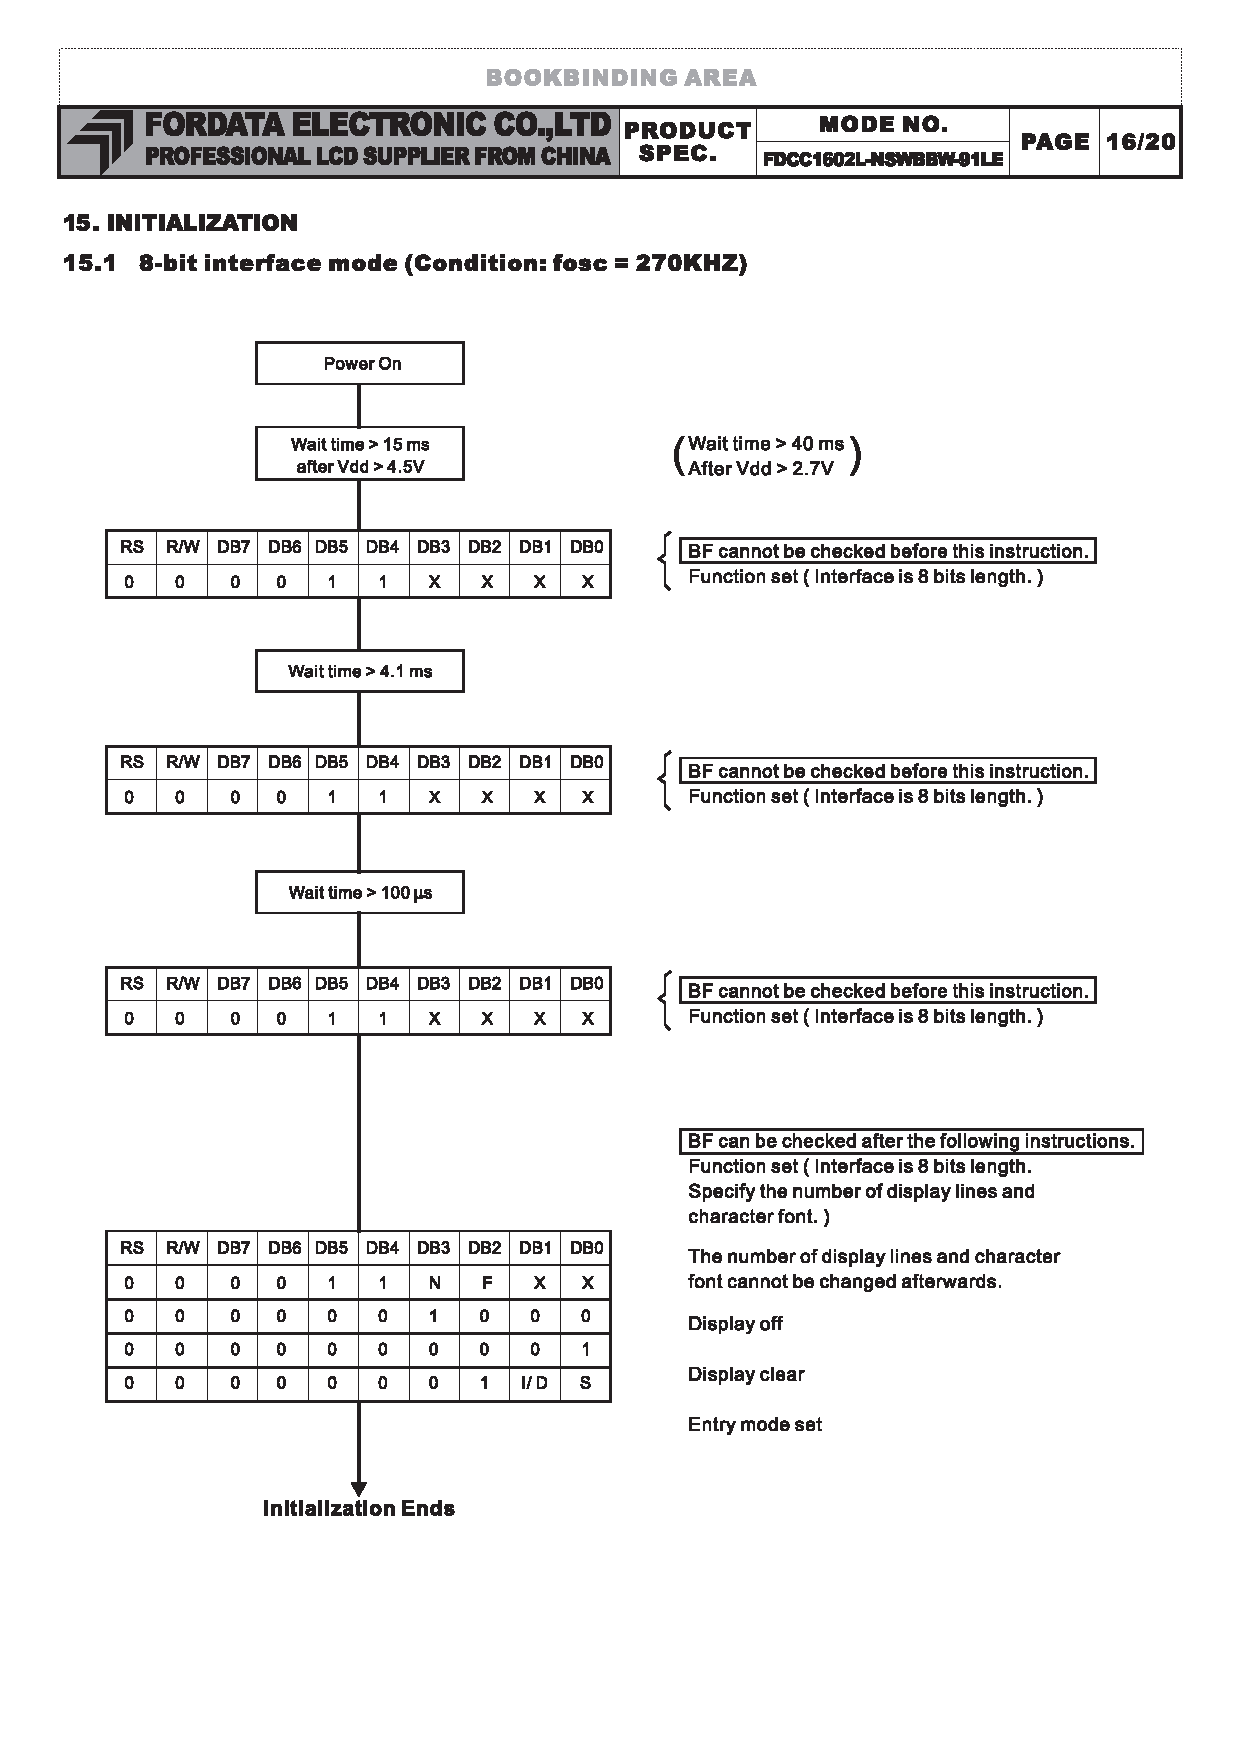
\includegraphics[width=\textwidth]{Images/InitalizationLCD8Bit}
	\caption{LCD Controller Initalization Sequenz}
	\label{image:lcdinit}
\end{figure}


\begin{lstlisting}[frame=htrbl, caption={Initalisierungssequenz des LCD-Controllers}, label={lst:lcdinit}]
void initMyLCD()
{
// 15mS delay after Vdd reaches nnVdc before proceeding with LCD initialization
// not always required and is based on system Vdd rise rate
uint16_t ui16I=0;
while(ui16I++<0xFFFF)Nop();

/* set initial states for the data and control pins */
DATA &= 0xFF00; //set RE0-RE7 low
RW = 0;                         // R/W state set low
RS = 0;                         // RS state set low
E = 0;                          // E state set low

/* set data and control pins to outputs */
TRISE &= 0xFF00;                //set RE0-RE7 to output
RW_TRIS = 0;                    // RW pin set as output
RS_TRIS = 0;                    // RS pin set as output
E_TRIS = 0;                     // E pin set as output

/* 1st LCD initialization sequence */
DATA &= 0xFF00;                 //set RE0-RE7 low
DATA |= 0x0038;                 //set lcd type: 8-bit,2lines,5x7
clockLCDenable();               // toggle E signal
ui16I=0; while(ui16I++<23256)Nop(); //5ms Delay

// 2nd LCD initialization sequence
DATA &= 0xFF00;
DATA |= 0x0038;
clockLCDenable(); 				// toggle Enable signal
ui16I=0; while(ui16I++<4651)Nop(); //200us Delay

// 3rd LCD initialization sequence
DATA &= 0xFF00;
DATA |= 0x0038;
clockLCDenable();
ui16I=0; while(ui16I++<4651)Nop(); //200us Delay

sendCommandLCD( 0x38 );         // function set 8bit, 2lines
sendCommandLCD( 0x0C );         // Display on control, cursor blink off (0x0C), cursor off
sendCommandLCD( 0x06 );         // entry mode set (0x06), increment cursor, no shift 
}
\end{lstlisting}
\newpage

\newpage
\begin{lstlisting}[frame=htrbl, caption={Funktionsprototypen edaPIC33LCD-Library}, label={lst:lcdlib}]
extern char ShadowString[32]; 

void initMyLCD();

void clockLCDenable();

void putcLCD(char c);

void putsLCD(char* pData);

void sendCommandLCD(uint8_t ui8data);

void sendCommandLCDNonBlocking(uint8_t ui8data);

void writeDataLCD(uint8_t ui8data);

void writeDataLCDNonBlocking(uint8_t ui8data);

void setDDRAMAddressLCD(uint8_t ui8address);

uint8_t readBusyFlagLCD();

void putncLCD(char* pData, uint8_t ui8n);

void SendDataToLCD();

void clearLCDStorage();

void SendDataToLCD();

void setLineLCD(const char* pStr, uint8_t ui8Line);

void setLCDLine1(const char* pString);

void setLCDLine2(const char* pString);

\end{lstlisting}
\newpage
